\documentclass{article}
\usepackage[utf8]{inputenc}
\usepackage{graphicx}
\usepackage{amsmath}
\usepackage{subcaption}
\usepackage{tabto}
\usepackage{multicol}


\title{Rendu Projet S5-17132}
\author{Durand Arthur /||/ Hamouche Luxel}
\date{January 2023}

\begin{document}


\maketitle Sommaire :
\begin{center}
  
\includegraphics[scale=0.6]{logo_em.jpg}  
\end{center}
\newpage
\section{Introduction}

\begin{itemize}
    \item  Présentation de l'équipe 
    \item Présentation du projet 
    \begin{itemize}
        \item Les règles du jeu
        \item Stratégies 
    \end{itemize}
\end{itemize}


\section{Parties du projets}

\begin{itemize}
    \item Environement de jeu (variable pions etc)
    \begin{itemize}
        \item Structure et Variables globales:
        \\
        La premiere chose à faire était de définir des constantes, stuctures et variables qui allait nous servire tout au long du projet tel que : \\
        Les directions :
        \\
        \begin{center}
        \begin{multicols}{2}
        
            NORTH \\ NEAST  \\ NWEST \\ WEST \\ SOUTH \\ SWEST \\ SWEST \\ EAST  
        
        \end{multicols}
        \end{center} 
        Le type de couleur de la case :
        \begin{center}
            NO-COLOR \hspace{1cm} WHITE \hspace{1cm} BLACK \\
        \end{center}
        L'occupant de la case :
        \begin{center}
            NO-SORT \hspace{2cm} SIMPLE-PAWN \\ 
        \end{center}
        Cette catégorie est voué à s'agrandir au vu de l'ajout de différentes sorte de pions par la suite. \\
        Egalement 
        \item Plateau : 
        \\
        Il faut definir un plateau de jeu pour l'utilisateur. Nous avons decidé de faire celui-ci de forme torique afin rendre le jeu plus modulable. Il a donc fallut nous affranchire des effets de bord à l'aide de modulo. Ce choix a aussi été fait pour des raisons d'entisipation des futures modifications qui seront plus faciles en partant d'un modèle très généraliste tel que le tore.\\
        \begin{center}
        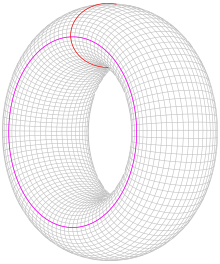
\includegraphics[scale=0.3]{220px-Torus_cycles2.svg.png}
        \end{center}
        
        
        Nous avons également pris par défault des relations entre les cases de type hexagonale comme il nous l'était imposé en début de projet. Cependant dans le cadre d'un achievement nous avons également implémenté un changement de térrain qui impact les relations faisant passer de case octogonale à des cases carré ou triagulaire. Ces changements arrivent tout les x tours en focntion de la demande du joueurs.
\begin{figure}[htbp]
\centering
\begin{subfigure}{0.3\textwidth}
\centering
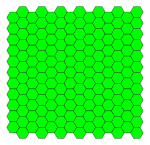
\includegraphics[width=\textwidth]{1-uniform_n1.svg.png}
\caption{Pavage hexagonale}
\label{label_de_l_image_1}
\end{subfigure}
\quad
\begin{subfigure}{0.3\textwidth}
\centering
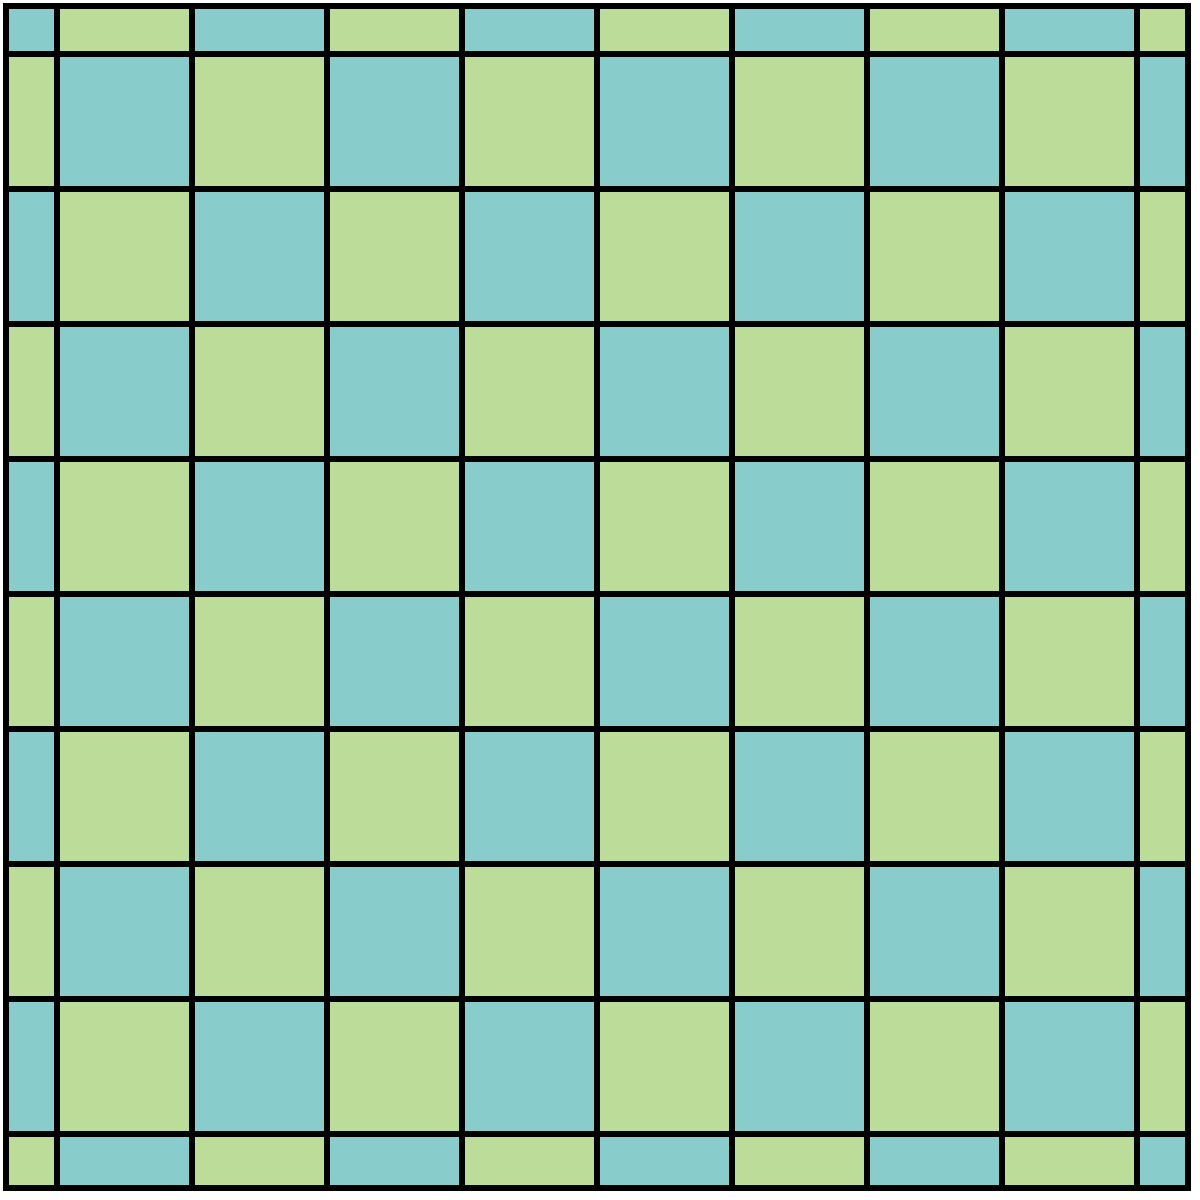
\includegraphics[width=\textwidth]{1200px-Tiling_Regular_4-4_Square.svg.png}
\caption{Pavage carré}
\label{label_de_l_image_2}
\end{subfigure}
\quad 
\begin{subfigure}{0.3\textwidth}
\centering
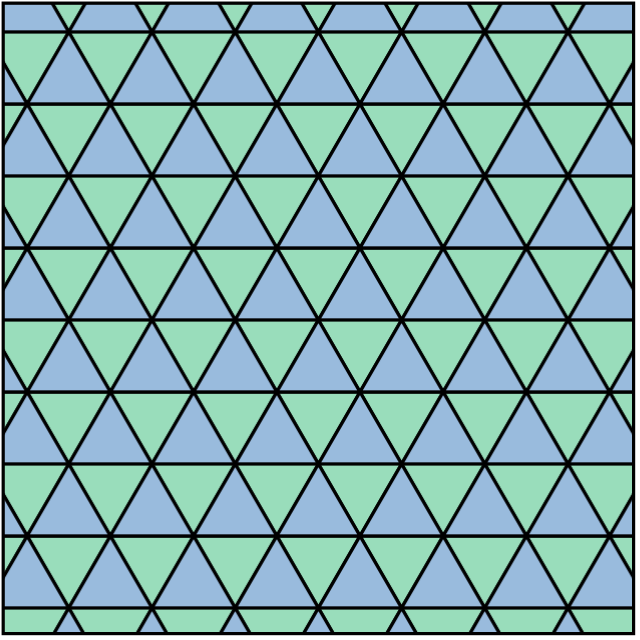
\includegraphics[width=\textwidth]{640px-Tiling_Regular_3-6_Triangular.svg.png}
\caption{Pavage Triangulaire}
\label{label_de_l_image_3}
\end{subfigure}
\caption{Pavages disponible dans notre jeu}
\label{label_de_la_figure 1}
\end{figure}

\newpage



        \item Pieces :
        \\
        Pour les pieces premièrement nous avons choisi de simple pions, pouvant se déplacer d'une seul case seulement si celle-ci est vide. Par la suite on a incorporé au jeu d'autres pieces le rendant plus interessant. Chaque piece a ses spécialités.  /
        La Tour : ( insérer image )\\
        Elle peut comme aux échecs se déplacer seulement en direction des points cardinaux. Nous avons décidé de limiter ses déplacement au Max(longueur du plateau, largeur du plateau) car tant donné l'apparence torique de notre plateau de jeux ses movements pourrait être infinies.  
        \item Joueurs
        \item Boucle de jeu
    \end{itemize}

    
    \item Architecture 
    \begin{itemize}
        \item Inclusion
        \item Complexité 
    \end{itemize}
    \item Tests 
    \begin{itemize}
        \item Structures Tests
        \item Notre utilisation des tests pour le bon focntionnement du projet 
    \end{itemize}
    \item Difficultées rencontrées 
    \end{itemize}

\section{Conclusion}
\begin{itemize}
    \item Points à amélioré

    \item Ce que le projet nous a apporté 
    \begin{itemize}
        \item Découverte de GitHub
        \item Découverte du Makefile
    \end{itemize}
\end{itemize}


\end{document}
